\chapter{Mathematical Foundations}
\epigraph{By relieving the brain of all unnecessary work, a good notation sets it free to concentrate on more advanced problems, and, in effect, increases the mental power of the race.}{Alfred North Whitehead}
  \section{3D Notation}

In this thesis, we largely follow the notation of \cite{Barfoot2017-ri} when dealing with three-dimensional rigid-body kinematics. As it is crucial to all four components of the work, we will begin by outlining the basic components.

\begin{figure}[h!]
\center
\tdplotsetmaincoords{60}{110}
%
\pgfmathsetmacro{\rvec}{1.75}
\pgfmathsetmacro{\thetavec}{45}
\pgfmathsetmacro{\phivec}{60}
%
\begin{tikzpicture}[scale=5,tdplot_main_coords]
\coordinate (O) at (0,0,0) node[anchor=south east]{$\CoordinateFrame{o}$};
\draw[very thick,->, red] (0,0,0) -- (0.7,0,0);
\draw[very thick,->, green] (0,0,0) -- (0,0.7,0);
\draw[very thick,->, blue] (0,0,0) -- (0,0,0.7);
\tdplotsetcoord{V}{\rvec}{\thetavec}{\phivec}
\tdplotsetrotatedcoords{\phivec}{\thetavec}{0} 
\tdplotsetrotatedcoordsorigin{(V)}

\draw [fill, tdplot_rotated_coords] (.3,.3,.3) circle [radius=0.01] node[anchor=north west]{$p$};
\draw[-stealth,tdplot_rotated_coords, black] (O) -- (.31,.31,.31) node[midway,below] {$\VectorArrow{r}^{po}$} ;


\end{tikzpicture}
\caption{A position vector expressed in a coordinate frame.}
\end{figure}

We refer to a three-dimensional position vector, $\VectorArrow{r}^{po}$, as one that originates at the origin of a coordinate reference frame, $\CoordinateFrame{o}$, and terminates at the point $p$. This geometric quantity has the numerical coordinates $\Vector{r}^{po}_o$ when expressed in $\CoordinateFrame{o}$. Often, we will refer to two reference frames such as a world or \textit{inertial} frame,  $\CoordinateFrame{i}$, and a vehicle frame, $\CoordinateFrame{v}$. Rotation matrices or rigid-body transformations that convert coordinates from $\CoordinateFrame{i}$ to $\CoordinateFrame{v}$ will be represented as $\Transform_{vi}$, and $\Rotation_{vi}$\footnote{We use $\Rotation$ and not $\Matrix{R}$ for rotation matrices to avoid confusion with common notation for measurement model covariance.}, respectively. 


\begin{figure}[h!]
\center
\tdplotsetmaincoords{60}{110}
%
\pgfmathsetmacro{\rvec}{1.75}
\pgfmathsetmacro{\thetavec}{45}
\pgfmathsetmacro{\phivec}{60}
%
\begin{tikzpicture}[scale=5,tdplot_main_coords]
\coordinate (O) at (0,0,0) node[anchor=south east]{$\CoordinateFrame{i}$};
\draw[very thick,->, red] (0,0,0) -- (0.7,0,0);
\draw[very thick,->, green] (0,0,0) -- (0,0.7,0);
\draw[very thick,->, blue] (0,0,0) -- (0,0,0.7);
\tdplotsetcoord{V}{\rvec}{\thetavec}{\phivec}
\draw[-stealth] (O) -- (V) node[midway,above] {$\VectorArrow{t}^{vi}$} ;

\tdplotsetrotatedcoords{\phivec}{\thetavec}{0} 
\tdplotsetrotatedcoordsorigin{(V)}


%Coordinate frame with label
\draw[very thick,tdplot_rotated_coords,->, red] (0,0,0) -- (.4,0,0);
\draw[very thick,tdplot_rotated_coords,->, green] (0,0,0) -- (0,.4,0);
\draw[very thick,tdplot_rotated_coords,->, blue] (0,0,0)-- (0,0,.4);
\draw[tdplot_rotated_coords] (0,0,0) node[anchor=south east] {$\CoordinateFrame{v}$};

%Local vector
\draw [fill, tdplot_rotated_coords] (.31,.31,.31) circle [radius=0.01] node[anchor=north west]{$p$};
\draw[-stealth,tdplot_rotated_coords, purple] (0,0,0) -- (.3,.3,.3) node[midway,above] {\footnotesize $\VectorArrow{r}^{pv}$};
\draw[-stealth,tdplot_rotated_coords, black] (O) -- (.3,.3,.3) node[midway,below] {$\VectorArrow{r}^{pi}$} ;

\end{tikzpicture}
\caption{Two common references frames used throughout this thesis.}
\end{figure}



\section{Rotations} 

The rotation matrix $\Rotation$ is a member of the matrix Lie group $\LieGroupSO{3}$ and can be defined as a matrix as follows:

\begin{equation}
\LieGroupSO{3} = \{ \Rotation \in \Real{}^{3 \times 3} | ~ \Rotation^T\Rotation = \Matrix{1}, \det{\Rotation} = 1  \}.	
\end{equation}

\subsubsection{Active vs. Passive}
An active (or alibi) rotation changes the coordinates of a position directly while implicitly assuming that the reference frame is fixed. A passive (or alias) rotation rotates the reference frame. Following \cite{Barfoot2017-ri}, all rotation matrices in this thesis are passive unless otherwise noted.  

\subsubsection{Exponential and Logarithmic Maps}

Since rotations form a matrix Lie group (we refer the reader to \cite{Sola2018-kg} and \cite{Barfoot2017-ri} for more thorough presentation of Lie groups), we can define a surjective exponential map\footnote{We follow \cite{Sola2018-kg} and also define \textit{capitalized} map for notational clarity.} from three axis-angle parameters, $\RotationVector = \phi \Vector{a}, ~~ \phi \in \Real{}, \Vector{a} \in S^2$, to a rotation matrix, $\Rotation$: 
\begin{align}
\label{eq:so3_exp}
\Rotation = \MatExp{\Vector{\phi}} = \Matexp{\Vector{\phi}} &= \sum_{n=0}^{\infty}  \frac{1}{n!} {(\Vector{\phi}^\wedge)}^n\\
\label{eq:euler_rodriguez}
&= \cos{\phi} \IdentityMatrix + (1 - \cos{\phi}) \Vector{a}\Vector{a}^T + \sin{\phi} \Vector{a}^\wedge,
\end{align}

where the wedge operator $(\cdot)^\wedge$\footnote{This operator is often expressed as $(\cdot)^\times$ and is known as the skew-symmetric operator.} is defined as
\begin{equation}
\Vector{a}^\wedge = \bbm a_0 \\ a_1 \\ a_2 \ebm^\wedge = \bbm 0 & -a_2 & a_1 \\ a_2 & 0 & -a_0 \\ -a_1 & a_0 & 0 \ebm.	
\end{equation}

\Cref{eq:euler_rodriguez} is known as the Euler-Rodriguez formula and it can also be derived geometrically, starting from Euler's theorem that any rotation can be expressed as an axis of rotation and an angle of rotation about that axis. Although  the map in \Cref{eq:so3_exp} is surjective, we can define an inverse map if we restrict its domain to $0 \leq \phi < \pi$:

\begin{align}
\label{eq:so3_log}
\RotationVector =  \MatLog{\Rotation} = \Matlog{\Rotation} &= \frac{\phi (\Rotation - \Rotation^T)^\vee}{2 \sin{\phi}}, 
\end{align}

where $\phi = \arccos{\frac{\Trace{\Rotation} - 1}{2}}$ and the \textit{vee} operator, $(\cdot)^\vee : \Real{}^{3 \times 3} \rightarrow \Real{}^3$, is defined as the unique inverse of the wedge operator $(\cdot)^\wedge$. Note \Cref{eq:so3_log} is undefined at both $\phi = 0$ and at $\phi = \pi$. In the former case, we can use a small-angle approximation and define

\begin{equation}
	\MatLog{\Rotation} \approx (\Rotation - \IdentityMatrix)^\vee ~~ \textrm{when} ~~ \phi \approx 0. 
\end{equation}

The latter case, (when $\phi = \pi$), defines the \textit{cut locus} of the space where $\MatExp{\cdot}$ is not a covering map and both $+\RotationVector$ and $-\RotationVector$ map to the same $\Rotation$. This \textit{cut locus} is related to the idea that any three parameterization of $\LieGroupSO{3}$ will have singularities associated with it.

\subsection{Unit Quaternions}

Another way (and historically, the original way) to represent a general rotation is to use a unit quaternion, $\quat$. A unit quaternion has four parameters, a scalar $q_\omega$ and a three-dimensional vector component, $\quat_v$:

\begin{equation}
	\quat = \bbm q_\omega \\ \quat_v \ebm \in S^3, ~~ (\Norm{\quat} = 1).
\end{equation}

Unit quaternions also form a Lie group \citep{Sola2018-kg} and and lie on a three-dimensional unit sphere within $\Real{}^4$. This manifold represents a double cover of $\LieGroupSO{3}$ (since both $\quat$ and $-\quat$ represent the same rotation). As with rotation matrices, we can define a surjective map from three parameters to the group itself,

\begin{equation}
\quat = \MatExp{\RotationVector} = \bbm \cos{\phi/2} \\ \Vector{a} \sin{\phi/2} \ebm.	
\end{equation}

Similarly, we can also define a logarithmic map,

\begin{align}
\label{eq:math_quat_log}
	\RotationVector =  \MatLog{\quat} = 2 \quat_v \frac{\arctan{(\Norm{\quat_v},  q_\omega})}{\Norm{\quat_v}}.
\end{align}

To avoid issues with the double cover, we replace $\quat$ with $-\quat$ if $q_\omega$ is negative before evaluating \Cref{eq:math_quat_log}. Also note again that \Cref{eq:math_quat_log} is undefined when $\phi = 0$, but, importantly, we do not face any issues when $\phi = \pi$ due to the half angle. As with rotation matrices, we can use small angle approximations to define:

\begin{equation}
	\MatLog{\quat} \approx \frac{\quat_v}{q_\omega} \left( 1 - \frac{\Norm{\quat_v}^2}{3 q_\omega^2}\right) ~~ \textrm{when} ~~ \phi \approx 0. 
\end{equation}

A fantastic summary of the history of rotation parameterizations, unit quaternions and the story of Hamilton and Rodriguez can be found in \cite{Altmann1989-ru}.



\section{Spatial Transforms}
The rigid body transform $\Transform_{vi}$ is a also a member of the matrix Lie group, $\LieGroupSE{3}$ and can be defined as a $4 \times 4$ matrix as follows:

\begin{equation}
\LieGroupSE{3} = \{ \Transform = \bbm \Rotation & \Vector{t} \\ \Vector{0}^T & 1 \ebm \in \Real{}^{4 \times 4} | ~  \Rotation \in \LieGroupSO{3},  \Vector{t} \in \Real{}^3  \}.
\end{equation}

As a member of a matrix Lie group

\begin{equation}
\Transform = \Matexp{\Vector{\xi}} = \sum_{n=0}^{\infty}  \frac{1}{n!} {(\Vector{\xi}^\wedge)}^n	
\end{equation}

and the map $\RealNumbers[6]\to\mathfrak{se}(3)$,
\begin{equation}
  \Vector \xi^\wedge \triangleq \bbm \Vector \rho \\ \Vector \phi \ebm ^\wedge = \bbm
  \Vector \phi^\wedge & \Vector \rho \\ \Transpose{\Vector{0}} &  0 \ebm.	
\end{equation}

The transform $\Transform_{vi}$ can be expressed as a $4 \times 4$ transformation matrix as

\begin{equation}
\Transform_{vi} = \bbm \Rotation_{vi} & \Vector{t}_v^{iv} \\ \Vector{0}^T & 1 \ebm,
\end{equation}

where $\Rotation \in \LieGroupSO{3}$ is a rotation matrix. This allows us to use the homogenous point representation for $\Vector{r}^{pi}_i$ and express the following relation:

\begin{equation}
	\bbm \Vector{r}^{pi}_v \\ 1 \ebm = \underbrace{\bbm \Rotation_{vi} & \Vector{t}_v^{iv} \\ \Vector{0}^T & 1 \ebm}_{\Transform_{vi}} \bbm \Vector{r}^{pi}_i \\ 1 \ebm
\end{equation}



This is equivalent to  

\begin{equation}
 \Vector{r}^{pi}_v =  \Rotation_{vi} \Vector{r}^{pi}_i + \Vector{t}_v^{iv}  
 \end{equation}









%\subsection{Uncertainty through noise injection}
%
%
%\begin{figure}[h!]
%\center
%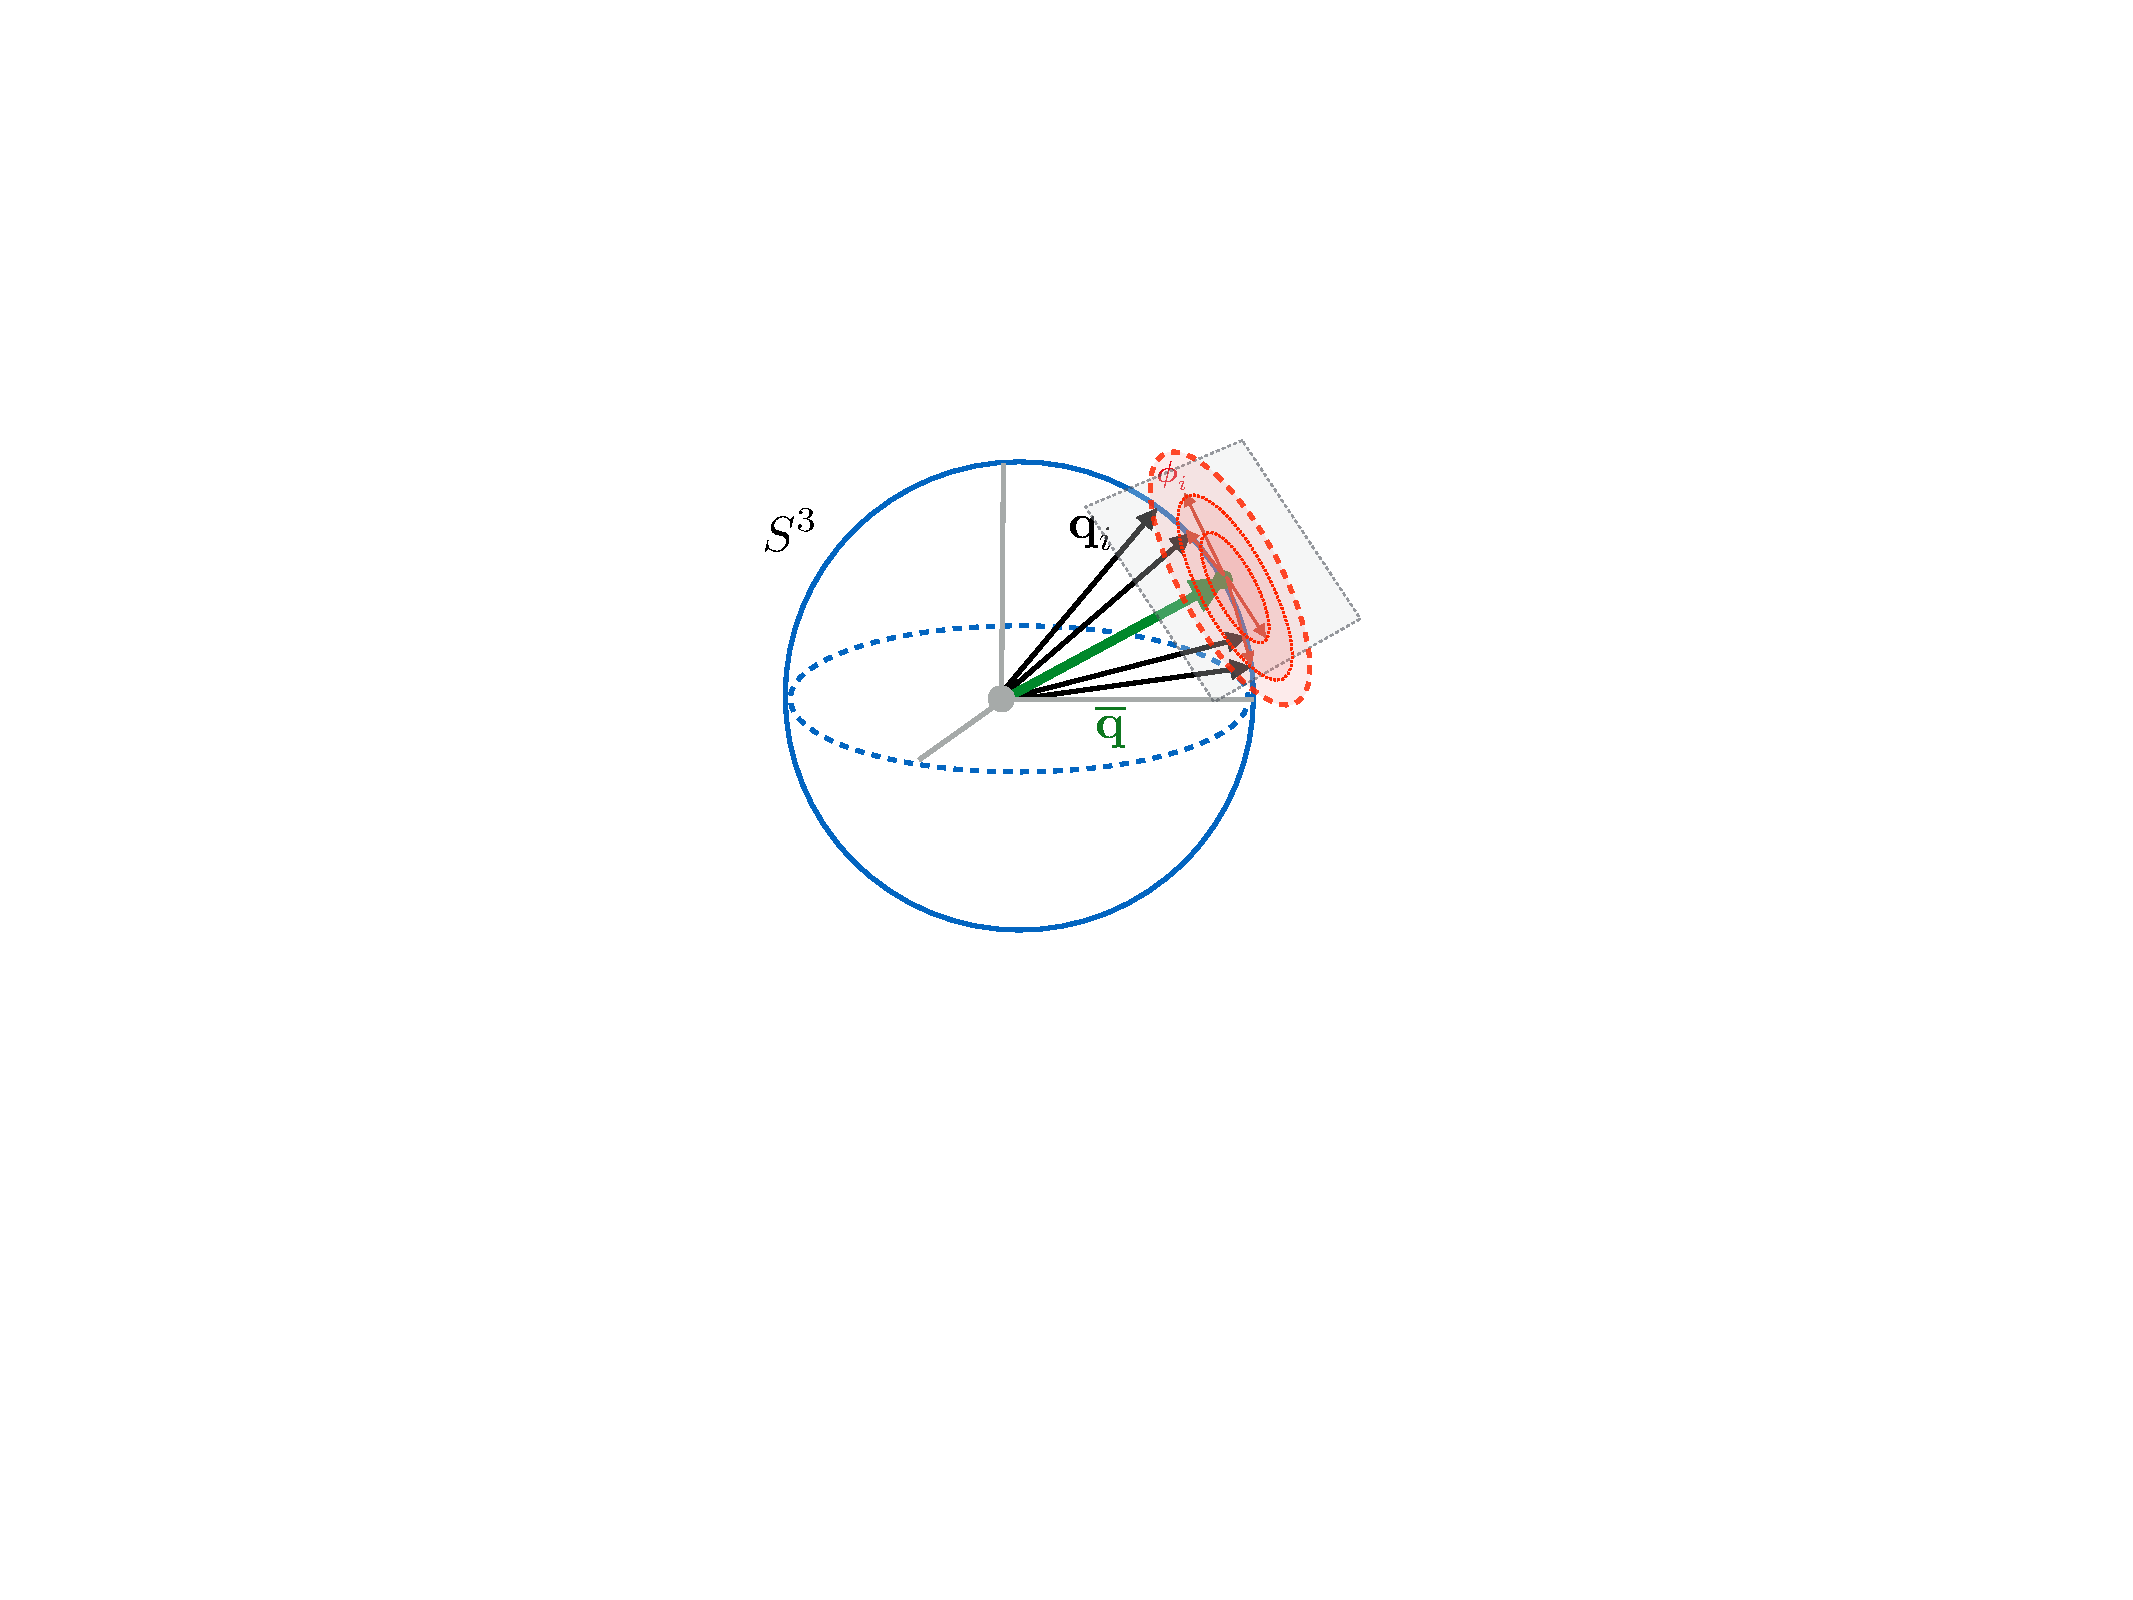
\includegraphics[width=0.3\textwidth]{math/quaternion_uncertainty}
%\caption{Uncertainty injection}
%\end{figure}

\section{Perturbations}

\todo{Left,middle,right}
\todo{Look at Seans thesis}


\section{Uncertainty}
\todo{Injection onto the manifold}


 